\chapter{Remote Method Invocation}
\section{Overview}
In modern, large distributed systems, nodes can be running in processes on several different physical machines. Using the Java Remote Method Invocation this can be done opaquely from the user. 

The Java RMI makes this possible. 

\section{Java RMI}

\subsection{Java Virtual Machine}

\subsection{Remote Method Invocation}

Remote Method invocation is an API integrated in the Java Virtual Machine which allows for remote procedure calls in an object-orientated manner. This is done by serializing java classes and transfering these to the remote location.

RMI is not to be confused with RPC (Remote procedure calls) since these are not object orientated.

Java RMI consists of three layers::

The \textbf{Stub and skeleton layer} are placed on either side of the whole network and transfer area. On the client side, a stub is created when a object is requested from the registry. When the client invokes a method on the stub, it communicates with a skeleton on the server side, which invokes the remote object.

The \textbf{Remote Reference layer} can be considered a middleware between the stub/skeleton layer and the transport layer. It handles references of remote objects, and manages creation, duplication and destruction of remote these objects. A Remote Reference manager (which is a sort of "controller" in this layer) is present both at the client and server side.

The \textbf{Transport layer} is responsible for network transfer. Here the TCP/IP connection is implemented. Here, the endpoints and incoming and outgoing connections is managed.

The coupling between the three layers is shown below:

\begin{center}
	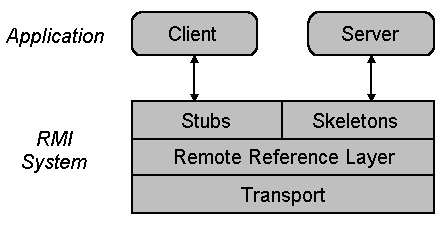
\includegraphics[scale=1.0]{RMI_layers.png}
    \captionof{figure}{RMI layers \cite{carleton}.}
\end{center}

\subsection{Serialization}

\subsection{The RMI Registry}

\section{Leader election}
\subsection{Overview}
In distributed systems, several different processes on several different machines can work together to solve a task or all be part of a major system.

In a larger system, it might very well be, that there has to be a leader to distribute work. The leader could also be the focal point for all other nodes in the system, granting access to some resource, database etc. 

\subsection{Leader Election}
If all nodes of the system are truly autonomous, each node's lifetime/stability should be completely decoupled from any other node. This provides an issue, if there is a leader in the system that goes down. 
The other nodes in the system must then, obscured from the user(s), \textit{elect} a new leader. The system should then resume, as if nothing had happened. 

In other words, the election of a new leader should happen as soon as it is discovered the current leader is irresponsive or faulty. There are several different algorithms for electing a new leader. In this report, two of these methods are discussed; The Bully election and the Ring election.

\subsection{Bully Election}

\subsection{Ring Election}
Ring election is , as the name says, leader election based on a ring. Contrary to Bully election, each note only communicates with the next in line.

Consider this figure:

\begin{center}
	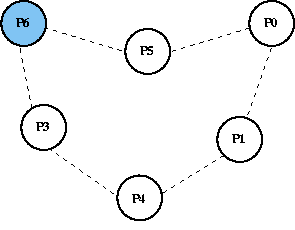
\includegraphics[scale=1.0]{RingElection_1.png}
    \captionof{figure}{Ring Leader Election \cite{colostate_RingElec}.}
\end{center}

Node number 6 crashes out, which leaves the system without a leader. When node number 3 tries to contact node 6, it realises that the leader has gone down, and it initialises a new election. A message is passed around the ring, and each node appends its own id to the list. When the message returns to node 3, it determines that it's id is already in the message, and the ring must be complete. Node 3 now determines the new leader. A message is sent around the ring, notifying everyone (including the new leader) who is the new leader. When this message reaches node 3 again, the node knows it has to stop it.\footcite{colostate_RingElec}

\begin{center}
	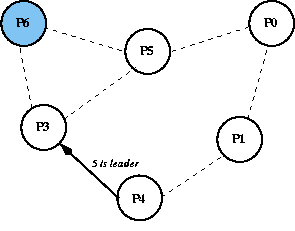
\includegraphics[scale=1.0]{RingElection_2.png}
    \captionof{figure}{Passing new leader message around \cite{DesignPatterns}}
\end{center} 
